\documentclass{beamer}

\usepackage[utf8]{inputenc} % Language and font encoding
\usepackage[icelandic]{babel}
\usepackage[T1]{fontenc}


\usepackage{tikz}
\usepackage[listings,theorems]{tcolorbox}
\usepackage{booktabs}
\usepackage{minted} %Minted and configuration
\usemintedstyle{default}

\renewcommand{\theFancyVerbLine}{\sffamily \arabic{FancyVerbLine}}
%%%%%%%%%%%
% More math
%%%%%%%%%%%
\newcommand{\Mod}[1]{\ \text{mod}\ #1}

%%%%%%%%%%%%%%%%%%%%%%
% Beamer configuration
%%%%%%%%%%%%%%%%%%%%%%
\setbeamertemplate{navigation symbols}{}
\usecolortheme{dove}
\setbeamercolor{frametitle}{fg=white}

\usebackgroundtemplate%
{%
\vbox to \paperheight{

\includegraphics[width=\paperwidth]{Pics/hi-slide-head-2016}

\vfill
\hspace{0.5cm}
\includegraphics[width=0.3\paperwidth]{Pics/hi-von-logo}
\vspace{0.4cm}
    }%
}

\AtBeginSection[]
{
  \begin{frame}<beamer>
    \frametitle{Yfirlit}
    \tableofcontents[currentsection]
  \end{frame}
}

\setbeamerfont{frametitle}{size=\normalsize}
\addtobeamertemplate{frametitle}{}{\vspace*{0.5cm}}

%%%%%%%%%%%%%%%%%%%%%%%%%
% tcolorbox configuration
%%%%%%%%%%%%%%%%%%%%%%%%%

% Setup from: http://tex.stackexchange.com/a/43329/21638
\tcbset{%
    noparskip,
    colback=gray!10, %background color of the box
    colframe=gray!40, %color of frame and title background
    coltext=black, %color of body text
    coltitle=black, %color of title text 
    fonttitle=\bfseries,
    alerted/.style={coltitle=red, colframe=gray!40},
    example/.style={coltitle=black, colframe=green!20, colback=green!5},
}


%%%%%%%%%%%%%%%%%%%%%%%
% Further configuration
%%%%%%%%%%%%%%%%%%%%%%%
\hypersetup{colorlinks=true,pdfauthor={Eirikur Ernir Thorsteinsson},linkcolor=blue,urlcolor=blue}
\graphicspath{{./Pics/}}

\author{Eiríkur Ernir Þorsteinsson}
\institute{Háskóli Íslands}
\date{Haust 2016}

\title{Tölvunarfræði 1a}
\subtitle{Vika 11, fyrri fyrirlestur}

\begin{document}

\begin{frame}
\titlepage
\end{frame}

\section{Inngangur}

\begin{frame}{Í síðasta þætti\ldots}
\begin{itemize}
 \item Hreiðruð föll
 \item Endurkvæmni
\end{itemize}
Kaflar: 10.4 - 10.5
\end{frame}

\begin{frame}{Næstu skilaverkefni}
\begin{itemize}
 \item Útlit er fyrir að við náum 12 skilaverkefnum
 \begin{itemize}
  \item Skilaverkefni 9: Skil 3. nóvember
  \item Skilaverkefni 10: Skil 10. nóvember 
  \item Skilaverkefni 11: Skil 17. nóvember
  \item Skilaverkefni 12: Skil 24. nóvember - spes skil
 \end{itemize}
 \item Af þessum 12 verkefnum mun einkunn 10 bestu skilaverkefna gilda 20\% til lokaeinkunnar
\end{itemize}
\end{frame}

\section{Hlutbundin forritun}

\begin{frame}{Hlutbundin forritun}
\begin{itemize}
 \item Hingað til höfum við verið að raða gögnunum okkar niður í vigra, hólfafylki, færslur\ldots
 \begin{itemize}
  \item Föll taka gögnin síðan inn, vinna með þau og skila öðrum gögnum
  \item Þessi forritunaraðferð er oftast kölluð ``procedural programming''
 \end{itemize}
 \item Hægt er að nálgast forritun á annan hátt - hlutbundinn (e. \emph{object oriented})
\end{itemize}
\end{frame}

\begin{frame}{Að forrita hlutbundið}
 \begin{itemize}
  \item Í procedural forritun byrjum við venjulega á að finna svör við spurningum á borð við
  \begin{itemize}
   \item Hvernig líta gögnin mín út?
   \item Hvernig get ég reiknað úr þessum gögnum?
  \end{itemize}
  \item Í hlutbundinni forritun þurfum við að svara aðeins öðrum spurningum
  \begin{itemize}
   \item Hvaða fyrirbrigði/hlutir koma við sögu í vandamálinu?
   \item Hvernig hegða þessir hlutir sér?
  \end{itemize}
 \end{itemize}
\end{frame}


\begin{frame}{Hvað er hlutur?}
\pause
\begin{itemize}
 \item Fyrirbrigði sem skilgreinast af gögnum og aðgerðum á þau geta verið hlutir
 \begin{itemize}
  \item Mjög opið hugtak! \pause
 \end{itemize}
 \item Dæmi um fyrirbrigði sem gætu verið hlutir í forriti? \pause
 \begin{itemize}
  \item Allt sem sést í tölvuleikjum
  \item Hringur
  \begin{itemize}
   \item Gögn/eiginleikar: Staðsetning miðpunkts, radíus
   \item Aðgerðir: Teikna, reikna flatarmál
  \end{itemize} 
  \item Almennt brot
  \begin{itemize}
   \item Gögn/eiginleikar: Nefnari, teljari
   \item Aðgerðir: Leggja saman, stytta
  \end{itemize}
 \end{itemize}
\end{itemize}
\end{frame}

\section{Teiknihlutir}

\begin{frame}[fragile]{Teiknihlutir}
\begin{itemize}
 \item Fyrstu hlutirnir sem við sjáum í Matlab eru venjulega teiknihlutir
 \item Við getum skoðað teiknihlut með því að búa einn slíkan til
\begin{minted}{matlab}
>> f = figure
>> whos f
\end{minted}
 \item Getum fengið alla eiginleika hans með \texttt{get} fallinu
\begin{minted}{matlab}
>> get(f)
\end{minted}
\end{itemize}
\end{frame}

\begin{frame}[fragile]{Eiginleikar teiknihluta}
Við getum náð í ákveðna eiginleika teiknihluta með \texttt{get} eða með því að nota punktvirkjann
\begin{minted}{matlab}
>> f = figure();
>> f.Color
ans =
    0.9400    0.9400    0.9400
>> get(f, 'Color')
ans =
    0.9400    0.9400    0.9400
\end{minted}
Yfirleitt er meira viðeigandi að nota punktvirkjann.
\end{frame}

\begin{frame}[fragile]{Eiginleikar teiknihluta}
Við getum breytt ákveðnum eiginleikum teiknihluta með fallinu \texttt{set} eða með því að nota punktvirkjann
\begin{minted}{matlab}
>> set(f, 'Color', [0.5 0.5 0.5])
>> f.Color = [0.5 0.8 0.2];
\end{minted}
Yfirleitt er meira viðeigandi að nota punktvirkjann.
\end{frame}

\begin{frame}[fragile]{Fyrirlestraræfing}
Skráið ykkur inn á \url{http://socrative.com/} og gerið fyrstu tvær spurningarnar.

Herbergisnúmer = \texttt{TOL105G2016}

Notendanafn = HÍ-tölvupóstfang
\end{frame}


\section{Okkar eigin hlutir}

\begin{frame}[fragile]{Hvernig búum við til hluti í Matlab?}
\begin{columns}
\column{0.5\textwidth}
\begin{itemize}
 \item Til að búa til hluti í Matlab notum við svokallaða klasa (e. \emph{classes})
 \item Matlab-klasi á heima í sér \texttt{.m} skrá. Hann inniheldur
 \begin{itemize}
  \item Eiginleika (e. \emph{properties}) sem lýsa gögnum klasans
  \begin{itemize}
   \item Þetta eru breytur
  \end{itemize}
  \item Aðferðir (e. \emph{methods}) sem lýsa því hvernig gögnin hegða sér
  \begin{itemize}
   \item Þetta eru föll
  \end{itemize}
 \end{itemize}
\end{itemize}
\column{0.5\textwidth}
\begin{minted}[frame=lines]{matlab}
classdef ClassName % Nafn

    properties
        % Eiginleikar hingað
    end
    
    methods
        % Aðferðir hingað
    end
    
end
\end{minted}

\end{columns}
\end{frame}

\begin{frame}[fragile]{Dæmi: Almennt brot}
\begin{minted}[frame=lines, fontsize=\small]{matlab}
classdef Fraction

    properties
        n % Teljari / numerator
        d % Nefnari / denomenator
    end
    
    methods
        function frac = Fraction(numerator, denomenator)
            frac.n = numerator;
            frac.d = denomenator;
        end
    end
    
end
\end{minted}

\end{frame}

\begin{frame}{Í Matlab}
\begin{center}
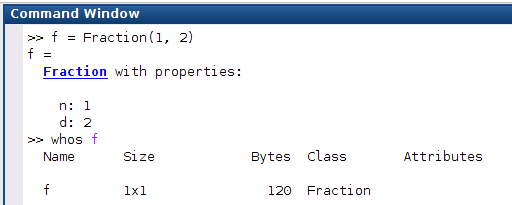
\includegraphics[width=\textheight]{Pics/fraction-workspace}
\end{center}
\end{frame}


\begin{frame}{Hvað vorum við að horfa á?}
\begin{itemize}
 \item Við vorum að skoða klasa með\ldots
 \item Tveimur eiginleikum
 \begin{itemize}
  \item \texttt{n} og \texttt{d}, sem tákna teljara og nefnara
  \item Einni aðferð, sem ``smíðar'' nýja hluti
  \begin{itemize}
   \item Slík aðferð er kölluð smiður (e. \emph{constructor})
   \item Notuð til að upphafsstilla gildi, athuga hvort að breyturnar séu af leyfilegum gerðum o.fl.
   \item Flestir klasar hafa smið
  \end{itemize}
 \end{itemize}
\end{itemize}
\end{frame}

\begin{frame}[fragile]{Fleiri aðferðir}
\begin{itemize}
 \item Getum bætt við fleiri aðferðum heldur en bara smiðnum
 \item Gætum bætt við aðferð sem heitir \texttt{simplify} sem einfaldar brotið sé kallað á það
 \item Aðferðir sem við skrifum geta ``yfirskrifað'' innbyggðar aðgerðir
 \begin{itemize}
  \item Getum yfirskrifað innbyggð föll m.t.t. klasans okkar
  \item Getum yfirskrifað innbyggða virkja
 \end{itemize}
\end{itemize}
\end{frame}


\begin{frame}[fragile]{disp-aðferð}
\begin{columns}
\column{0.45\textwidth}
\begin{itemize}
 \item Oftast viljum við að klasarnir okkar prentist á skynsamlegan hátt út þegar við köllum á \texttt{disp} eða þegar við gefum breytum gildi af hans tagi
 \item Hvernig gerum við það?
 \begin{itemize}
  \item Bætum við \texttt{disp} aðferð á klasann!
 \end{itemize}
\end{itemize}
\column{0.55\textwidth}

\begin{minted}[frame=lines, fontsize=\small]{matlab}
function disp(fr)
    fprintf('%d/%d\n', fr.n, fr.d)
end
\end{minted}

Þetta fer inn í ``\texttt{methods}'' blokk klasans
\end{columns}
\end{frame}

\begin{frame}{Yfirskrifun virkja}
Hver virki í Matlab samsvarar einu falli (\href{https://se.mathworks.com/help/matlab/matlab_oop/implementing-operators-for-your-class.html\#br02znk-6}{listi}). Dæmi:
\begin{center}
\begin{tabular}{ll}
\toprule
Virki&Fall\\
\midrule
$a+b$&\texttt{plus(a,b)}\\
$a-b$&\texttt{minus(a,b)}\\
$a*b$&\texttt{mtimes(a,b)}\\
$a/b$&\texttt{mrdivide(a,b)}\\
\bottomrule
\end{tabular}
\end{center}
Þessa virkja má útfæra fyrir klasa sem við skrifum.
\end{frame}


\begin{frame}[fragile]{Látum klasann vinna vinnu}
Við kunnum að leggja saman brot:
\[
\frac{c}{d} + \frac{a}{b} = \frac{cb+ad}{db} 
\]
Þetta má gera í klasanum okkar með því að bæta við aðferðinni
\begin{minted}[frame=lines]{matlab}
function newFrac = plus(frac1, frac2)
    newN = frac1.n * frac2.d + frac2.n * frac1.d;
    newD = frac1.d * frac2.d;
    newFrac = Fraction(newN, newD);
end
\end{minted}

Þessi aðferð yfirskrifar innbyggða plús-virkjann!
\end{frame}

\begin{frame}[fragile]{Fyrirlestraræfing}
Skráið ykkur inn á \url{http://socrative.com/} og klárið æfinguna.

Herbergisnúmer = \texttt{TOL105G2016}

Notendanafn = HÍ-tölvupóstfang
\end{frame}


\end{document}
